\documentclass[convert={density=300,size=1080x800,outext=.png}]{standalone}
\usepackage{tikz}
\usetikzlibrary{decorations.pathreplacing}
\begin{document}

%.. tikz:: 
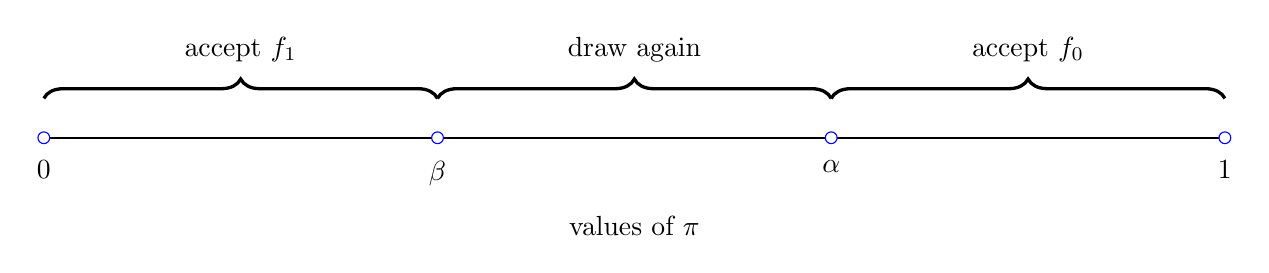
\begin{tikzpicture}
[scale=5, every node/.style={color=black}, decoration={brace,amplitude=7pt}] \coordinate (a0) at (0, 0.0);
    \coordinate (a1) at (1, 0.0);
    \coordinate (a2) at (2, 0.0);
    \coordinate (a3) at (3, 0.0);
    \coordinate (s0) at (0, 0.1);
    \coordinate (s1) at (1, 0.1);
    \coordinate (s2) at (2, 0.1);
    \coordinate (s3) at (3, 0.1);
    % axis
    \draw[thick] (0, 0)  -- (3, 0) node[below] {};
    %curly bracket
    \draw [decorate, very thick] (s0) -- (s1)
        node [midway, anchor=south,  outer sep=10pt]{accept $f_1$};
    \draw [decorate, very thick] (s1) -- (s2)
        node [midway, anchor=south, outer sep=10pt]{draw again};
    \draw [decorate, very thick] (s2) -- (s3)
        node [midway, anchor=south, outer sep=10pt]{accept $f_0$};
    \node[circle, draw, thin, blue, fill=white!10, scale=0.45] at (a0){};
    \node[below, outer sep=5pt] at (a0){$0$};
    \node[circle, draw, thin, blue, fill=white!10, scale=0.45] at (a1){};
    \node[below, outer sep=5pt] at (a1){$\beta$};
    \node[circle, draw, thin, blue, fill=white!10, scale=0.45] at (a2){};
    \node[below, outer sep=5pt] at (a2){$\alpha$};
    \node[circle, draw, thin, blue, fill=white!10, scale=0.45] at (a3){};
    \node[below, outer sep=5pt] at (a3){$1$};
    \node[below, outer sep=25pt] at (1.5, 0){values of $\pi$};
\end{tikzpicture}

\end{document}